\documentclass[crop, tikz]{standalone}
\begin{document}
	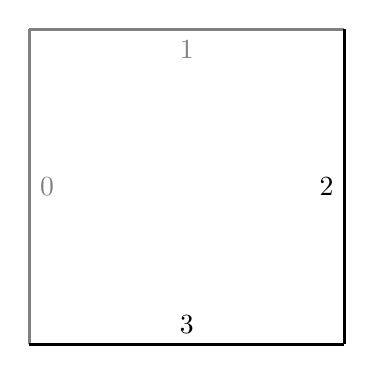
\begin{tikzpicture}
		\coordinate (A1) at (0, 0);
		\coordinate (A2) at (0, 4);
		\coordinate (A3) at (4, 4);
		\coordinate (A4) at (4, 0);
		
		\draw [very thick, auto=right, color= gray] 
		(A1) -- node {$0$} (A2) ;
		\draw [very thick, auto=right, color= gray] (A2)	-- node {$1$} (A3) ;
		\draw [very thick, auto=right] (A3)	-- node {$2$} (A4); 
		\draw [very thick, auto=right] (A4) -- node {$3$} (A1); %pretty corner
	\end{tikzpicture}
\end{document}